% Main chapter title
\chapter{Hauptkomponentenanalyse}

% Chapter label
\label{pca}

Die Hauptkomponentenanalyse ist ein weitverbreitetes multivariates statistisches Verfahren zur Dimensionsreduktion. Multivariate Verfahren zielen darauf ab, die in einem Datensatz enthaltene Zahl der Variablen zu verringern, ohne die darin enthaltene Information (zu verlieren) / (wesentlich zu reduzieren). Dadurch können umfangreiche Datensätze strukturiert, veranschaulicht und vereinfacht werden. Somit ist das Verfahren Teil der explorativen Statistik, welche Datensätze hinsichtlich ihrer Zusammenhänge analysiert.

So ist man meist besonders an der Bildung sog. Cluster, also Gruppierungen, interessiert. Datenpunkte, die im entstehendem Bild nach Anwendung der Hauptkomponentenanalyse nah beieinander liegen, sind in gewisser Weise ähnlich zueinander während Datenpunkte, die weit von einander entfernt liegen, wenig Ähnlichkeit aufweisen. Abbildung CITE zeigt die Entstehung solcher Cluster auf dem Datensatz. Mit diesem Verfahren lässt sich daher eine Art Struktur in den Daten erkennen, die für weitere Analysezwecke ausgenutzt werden kann.

So hat die Hauptkomponentenanalyse in vielen Bereichen erfolgreich Anwendung gefunden. Darunter fällt die Erkennung handgeschriebener Zahlen, welche zum Beispiel zur automatischen Sortierung von Briefen nach Postleitzahl genutzt wird \cite{hastie_elements}. Hier lässt sich die Bedeutung der Cluster besonders gut verdeutlichen. Man erhofft, dass nach Anwendung einer Transformation 10 verschiedene Gruppierungen zu erkennen sind, die für die Ziffern 0 bis 9 stehen. Optimalerweise gehören alle Datenpunkte im demselbem Cluster zur selben Ziffer. Außerdem korrespondieren nahe beieinanderliegende Cluster mit Ziffern, die ähnlich aussehen. Des Weiteren wird das Verfahren auch in der Gesichtserkennung CITE oder in der Genexpressionsanalyse genutzt CITE.

Das dahinterstehende mathematische Problem kann auf verschiedene Weisen beschrieben werden. Zunächst wollen wir die Hauptkomponentenanalyse so konstruieren, dass die Idee des minimalen Informationsverlust im Vordergrund steht. Anschließend werden wir das Problem auf eine Singulärwertzerlegung zurückführen, die auch zur effizienten Implementierung genutzt wird. Des Weiteren werden wir die Hauptkomponentenanalyse als Regressionsproblem betrachten und die geometrische Interpretation weiter verdeutlichen. Zu Schluss werden wir einige theoretische Aussagen zeigen.

\section{Konstruktion}

Gegeben sei ein Datensatz mit $n$ samples und $p$ Variablen. Die zentrale Idee der Hauptkomponentenanalyse besteht darin, die $p$ bestehenden Variablen in $r$ neue, unkorrelierte Variablen zu überführen. Um eine Reduktion der Dimension, also $r < p$ zu erreichen, müssen die bestehenden Variablen \textit{zusammengefasst} werden. Idealerweise sollte bei diesem Prozess möglichst wenig Information verloren gehen. Als Maß für den Informationsgehalt der Daten wird hierbei die Varianz verwendet. Das heißt, je größer die Varianz einer Variable, desto mehr Information birgt sie und desto \textit{wichtiger} ist sie. Hätte man eine Variable, die für alle Beobachtungen ähnliche Werte hat, so ist Diese nicht von Nutzen bei der Unterscheidung verschiedener samples. PCA sucht also nach Eigenschaften, die viel Varianz zeigen. Dabei wählt PCA aber nicht einfach nur bestimmte Eigenschaften mit viel Varianz aus, sondern konstruiert neue Variablen, die die bestehenden zusammenfassen.

Konkret suchen wir also sukzessive nach einer Linearkombination der bestehenden Variablen. Die entstehenden Vektor zeigen dann in die Richtung größter Varianz in unserem Datensatz. Wir nennen sie die Hauptachsen bzw. Hauptrichtungen unseres Datensatzes. Nachdem wir Diese berechnet haben wollen wir unsere Beobachtungen bezüglich der neuen Variablen darstellen. Dazu verwenden wir die orthogonale Projektion. Dies entspricht einer Rotation des Koordinatensystems, so dass die Hauptrichtugen den Standardachsen entsprechen. Die so entstehenden Werte bezüglich der neuen Variablen werden Hauptkomponenten genannt. 

Abbildung Höhe Gewicht mit Eigenvektoren und gedrehtes Bild

Um dieses Prinzip zu veranschaulichen, wenden wir uns nun einem simplem Beispiel zu. Gegeben seien die Größe [cm] und das Gewicht [kg] zu 1000 Personen (Daten sind simuliert, keine real-world-data) (siehe dazu Abbildung). In diesem Fall ist also $n = 1000$ und $p = 2$. Bei Betrachtung der Abbildung fällt schnell auf, dass die beiden Variablen positiv korreliert sind, d.h. prinzipiell gibt es die folgende Tendenz: Je größer eine Person, desto schwerer ist sie. Wir können

Konkret konstruieren wir Variablen, die sich aus Linerakombinationen der Alten zusammensetzen. Dabei sollen die neuen Variablen der Wichtigkeit nach sortiert sein. In anderen Worten enthält die erste Variable die meiste Information bzw. die größte Varianz, dann die zweite, usw.

Abbildung Scree Plot

Die eigentliche Dimensionsreduktion findet dann durch Selektierung statt. Je nach Komplexität des Modells und Informationsverlust können so mehr oder weniger ausgewählt werden. Somit haben wir eine kleine, neue Menge an Variablen, die aber trotzdem den Großteil an Informationen / Varianz beinhaltet. Anordnung nach absteigender Varianz bzw. Information.

Bevor wir die Hauptkomponentenanalyse auf den Datensatz anwenden können gibt es noch einen wichtigen Bearbeitungsschritt zu beachten. Wenn eine Variable weniger variiert als eine Andere aufgrund der verwendeten Einheit oder Skala (meter oder kilo) kann dies zu ungewollten Ergebnissen führen. Ohne eine Vorbehandlung der Daten hat so im obigen Beispiel eine Änderung von 1m die gleiche Bedeutung wie eine Änderung von 1kg. Allerdings ist ein Mensch, der 1m größer ist, ein ganz Anderer während ein Mensch, der 1kg mehr wiegt, noch sehr ähnlich ist. Daher werden die Daten häufig einem sog. preprocessing unterzogen. Ein zu diesem Zweck oft verwendetes Verfahren ist die Standardisierung (auch z-Transformation genannt). In diesem Schritt werden die Variablen so transfomiert, dass sie "vergleichbarer" werden. Seien dazu $X_i$ die Zufallsvariablen mit Erwartungswert $E[X_i] = \mu$ und Varianz $Var[X_i] = \sigma^2$. So erhält man die zugehörigen standardisierten Zufallsvariablen $Z_i$ durch Zentrierung und anschließender Division durch die Standardabweichung $Z = \frac{X-\mu}{\sigma}$. Somit gilt:
\begin{itemize}
\item $E[Z_i] = 0$ für alle $1 \leq i \leq p$
\item $Var[Z_i] = 1$ für alle $1 \leq i \leq p$
\end{itemize}
Mathematisch gesehen endet man das Verfahren also nicht auf die Kovarianzmatrix, sondern auf die Korrelationsmatrix an.

\subsection{Problemformulierung als Varianzmaximierung}

Wir wollen nun die Intuition des minimalen Informationsverlust mathematisch formulieren. Gegeben sei dazu eine Matrix $\mat{X} \in \mathbb{R}^{n\times p}$, wobei $n$ die Anzahl der Samples bzw. Beobachtungen und $p$ die Anzahl der Variablen ist. Wir nehmen im Folgenden ohne Beschränkung der Allgemeinheit an, dass die Variablen zuvor zentriert wurden. 

Aufgabe der Hauptkomponentenanalyse ist es nun sukzessive Richtungen größter Varianz zu finden. Wir bezeichnen die Hauptachsen mit $v_i$, wobei $v_i = (v_{i1}, \ldots, v_{ip})^T$. Die Darstellung der Beobachtungen bezüglich der neuen Variablen Hauptkomponenten $Z_i $werden dann durch d ist dann die Transformation dwird definiert durch $Z_i = \sum_{j=1}^p v_{ij}X_j = \mat{X}v$ wobei  so gewählt wird, dass die Varianz der ersten Hauptkomponente $Z_1$ maximiert wird:
$$v_1 = \argmax_{\norm{v}_2 = 1} \text{Var}[\mat{X}v] = \argmax_{\norm{v}_2 = 1} \frac{1}{n-1} v^T\mat{X}^T\mat{X}v  = \argmax_{\norm{v}_2 = 1} v^T \mat{K}_{xx} v$$
wobei $\mat{K_{xx}}$ die Kovarianzmatrix ist. Die erste Hauptkomponente, d.h. die Projektion der Daten auf die erste Hauptachse erhält man durch $Z_1 = \sum_{j=1}^{p} v_{1j}X_j$, wobei $v_1 = (v_{11}, \ldots, v_{1p})^T$. Die restlichen Hauptachsen und Komponenten können sukzessive definiert werden.
$$v_{k+1} = \argmax_{\norm{v} = 1} v^T \mat{K}_{xx} v$$ unter der Nebenbedingung, dass $v_{k+1}^Tv_l = 0, \forall 1 \leq l \leq k$. Man sucht also unter den Richtungen, die orthogonal zu allen bisherigen Hauptachsen sind, diejenige, die die Varianz maximiert.
\cite{zou_overview}
CITE JOLLIFE
und anschließend die Daten auf die neu konstruierten Variablen zu projizieren
Wie wir bereits in THEOREM gesehen haben, entsprechen die Eigenvektoren der Kovarianzmatrix genau den Richtungen maximaler Varianz wie oben definiert. Daher können wir anstatt sukzessiver Berechnung einzelner Hauptachsen die Kovarianzmatrix $\mat{K}_{xx}$ diagonalisieren. Da $\mat{K}_{xx}$ symmetrisch ist
$$\mat{K}_{xx} = \mat V \mat L \mat{V}^T$$
wobei $\mat V$ die Matrix der Eigenvektoren ist (Jede Spalte ist ein Eigenvektor) und $\mat{L}$ ist eine Diagonalmatrix mit Eigenwerten $\lambda_i$ in absteigender Reihenfolge. Die Eigenvektoren entsprechen den Hauptachsen und die Projektion der Daten auf die Hauptachsen wird erreicht durch Multiplikation des Datensatz mit den Eigenvektoren $\mat Z = \mat X \mat V$. Die Spalten in $\mat{Z}$ sind also die Hauptkomponenten. Die i-te Beobachtung bezüglich der neuen Variablen sind die Zeilen von $\mat{X}\mat{V}$.



 Wie wir bereits in CITE gesehen haben, entsprechend diese Richtungen genau den Eigenvektoren der Stichprobenkovarianzmatrix. Die Stichprobenkovarianzmatrix ist gegeben durch $\mat{K}_{xx} = \frac{(\mat{X}^T\mat{X})}{n}$. 
 


\subsection{Formulierung als Singulärwertzerlegung}
$$ \mat{X} = \mat{U}\mat{D}\mat{V}^T $$
wobei $\mat{D}$ eine Diagonalmatrix mit Elementen $d_1,\ldots,d_p$ in absteigender Reihenfolge, $\mat{U}$ eine $n \times p$ und $\mat{V}$ eine $p \times p$ orthogonale Matrix.
$\mat{U}\mat{V}$ sind die Hauptkomponenten und die Spalten von $\mat{V}$ sind die Eigenvektoren von $\mat{X}$.

\subsection{Formulierung als Regressionsproblem}

\begin{figure}
\centering
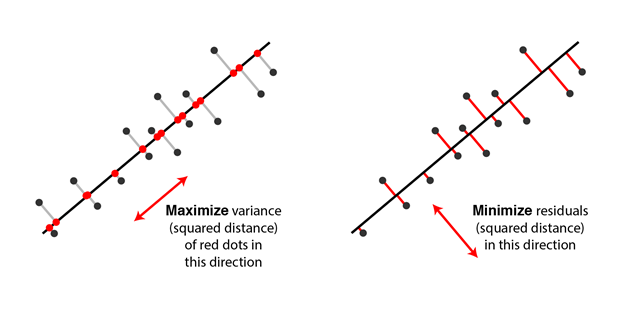
\includegraphics[width = 0.8\textwidth]{figures/pca_projection_explanation.png}
\caption{Die obenstehende Abbildung zeigt die Äquivalenz von Maximierung der Varianz und Minimierung der Projektionsdistanz}
\label{pca_projection_explanation}
\end{figure}

$$\hat{\mat{V}_k} = \argmin_{\mat{V}_k} \sum_{i=1}^{n} \norm{x_i - \mat{V}_k \mat{V}_k^Tx_i}^2 + \lambda \sum_{j=1}^{k}\norm{\beta_j}^2$$

subject to $\mat{V}_k^T\mat{V}_k = I_{k \times k}$

Wie bereits erwähnt (Wurde es erwähnt?) ist PCA ein lineares Dimensionsreduktionsverfahren, d.h. dass die Daten in den niedrigdimensionalen Raum linear, also durch eine Kombination von Rotationen und Translationen, transformiert / projeziert  werden. 

\cite{zou_sparsepca}

Man projiziert die Daten auf einen k-dimensionalen linearen Unterraum. Man kann zeigen, dass die Lösung dieses Problem genau die ersten k Hauptachsen sind.

Ausgehend von dieser Formulierung als Regressionsproblem werden wir im nächsten Kapitel die Variante der dünnbesetzten Hauptkomponentenanalyse beschreiben.

\section{Dimensionsreduktion}
Wie viele Hauptkomponenten sollen wir auswählen?

\section{Grenzen der Anwendbarkeit}

Obwohl die Hauptkomponentenanalysen in vielen Situationen helfen kann, Datensätze zu veranschaulichen und zu strukturieren, gibt es keine Garantie für sinnvolle Ergebnisse. Im Folgendem werden wir Szenarien beschreiben, bei denen unerwünschte Effekte bei der Verwendung dieses Verfahrens auftreten. Daher gilt es den Datensatz vorest hinsichtlich folgender Gesichtspunkte zu untersuchen: 

\begin{itemize}
\item Lineare Beziehung zwischen Variablen
\item Korrelation der Variablen
\item Vollständigkeit des Datensatzes
\item Ausreißer in den Daten
\item Anzahl an Beobachtungen in Relation zu Anzahl an Variablen
\end{itemize}

Wie in REF beschrieben versuchen wir Daten in einen niedrigdimensionaleren linearen oder affinen Unterraum zu transformieren. Es kann aber durchaus vorkommen, dass es keine lineare Beziehung zwischen den Variablen gibt. Nichtlineare Strukturen können von PCA nicht erfasst werden und gehen somit verloren. \cite{vidal} Vidal et al. zeigen diese Grenze konkret am Beispiel von Porträt-Fotos auf. Seit der Entstehung von PCA gab es aber zahlreiche nicht-lineare Erweiterungen. So nutzt zum Beispiel Kernel PCA den \textit{Kernel Trick} aus, bei welchem man die Daten zuerst durch eine nichtlineare Transformation in ein höherdimensionalen Raum einbettet von dem man sich erhofft, dass die Daten in diesem linear verteilt. Erst anschließend wird dann die eigentliche Reduktion durchgeführt. Hierbei muss man die Daten aber nicht im höherdimensionalen Raum auswerten. CITE. Andere Erweiterungen, die allgemein unter \textit{manifold learning} zusammengefasst werden können, basieren auf der Idee, dass die Dimension des Datensatz nur künstlich hoch ist. Man versucht die lokale Geometrie der Mannigfaltigkeit (Begriff erklären?) zu approximieren und damit direkt eine niedrigdimensionale Einbettung zu erhalten. Hierunter fallen zum Beispiel die multidimensionale Skalierung oder ISOMAP.

Damit der Datensatz für eine Dimensionsreduktion per PCA geeignet ist, müssen die verschiedenen Variablen einen gewissen Grad an Korrelation aufweisen. Im extremen Fall der Unabhängigkeit der Variablen bewirkt eine Hauptachsentransformation nichts. Reduziert man dann die Anzahl der Hauptkomponenten verliert man mit jeder Variable einen Großteil der Information.

Ein weiterer Gesichtspunkt ist die Vollständigkeit eines Datensatzes. Finden wir fehlende oder korrupte Einträge in unserem Datensatz vor, kann die klassische Hauptkomponentenanalyse ... . Für dieser Art Probleme existieren entsprechende Ergänzungen von PCA wie zum Beispiel in cite und cite. Ausreißer in den Daten können die Resultate drastisch beeinflussen. Genaue Effekte überlegen und CITE. Aus diesem Grund sollten Ausreißer vor der Anwendung von PCA entfernt werden.

Außreiser in den Daten.

Anzahl der Variablen zu hoch.

Darüber hinaus gibt es noch eine Reihe Spezialfälle, bei denen Probleme auftreten können. So kann es zum Beispiel passieren, dass die relevanten Informationen in den Variablen mit niedriger Varianz versteckt sind. Da die Hauptkomponentenanalyse gerade diese Variablen vernachlässigt, wird sich unter Umständen nicht die erwünschte Struktur auf den Daten ergeben. Es bedarf anderer Methoden mit anderen Ansätzen, um eine Dimensionsreduktion zu ermöglichen. Oftmals weiß man aber im Vorhinein nicht, in welchen Variablen diese Unterscheidungsmöglichkeit versteckt ist.

Das wohl wichtigste/größte Hindernis im Zuge dieser Arbeit ist sicherlich die durch die Transformation entstehenden Interpretationsschwierigkeiten. Jede Hauptkomponente entsteht wie oben beschrieben durch eine Linearkombination der Ausgangsvariablen. Während die Ausgangsvariablen Bedeutungen wie Gewicht oder Größe hatten ist in vor allem in hochdimensionalen Fällen eine Interpretation der Hauptkomponenten nur schwer möglich (Rotation Techniques CITE). Dieser Interpretationsverlust ist Ausgangspunkt der Idee der dünnbesetzten Hauptkomponentenanalyse, genannt sparse PCA. Diesem Verfahren ist das folgende Kapitel gewidmet.


\section{Theoretische Aussagen}

\begin{thm}
PCA always gives unique solution.
\end{thm}

\begin{thm}[\cite{vidal}]
Sei $\mat X \in \mathbb{R}^n$ und $\mat A_{p,k} = [\alpha_1, \ldots \alpha_k] $   
\end{thm}

\begin{thm}
PCA inconsistent for p >> n.
\end{thm}

